\section{Data Wrangling}

\subsection{Dataset}

\subsubsection{CelebA} \label{sec:CelebA}

CelebA is a large-scale face attributes dataset with more than 200K celebrity images, each with 40 attribute annotations. The images in this dataset cover large pose variations and background clutter. CelebA has large diversities, large quantities, and rich annotations, including \textbf{5,000 celebrity identities}, \textbf{202,599 face images}, and \textbf{40 binary attributes} annotations per image. The dataset can be employed as the training and test sets for the following computer vision tasks: face attribute recognition, face detection, landmark (or facial part) localization, and face editing/synthesis.

% insert the image of the dataset
\begin{figure}[h]
\centering
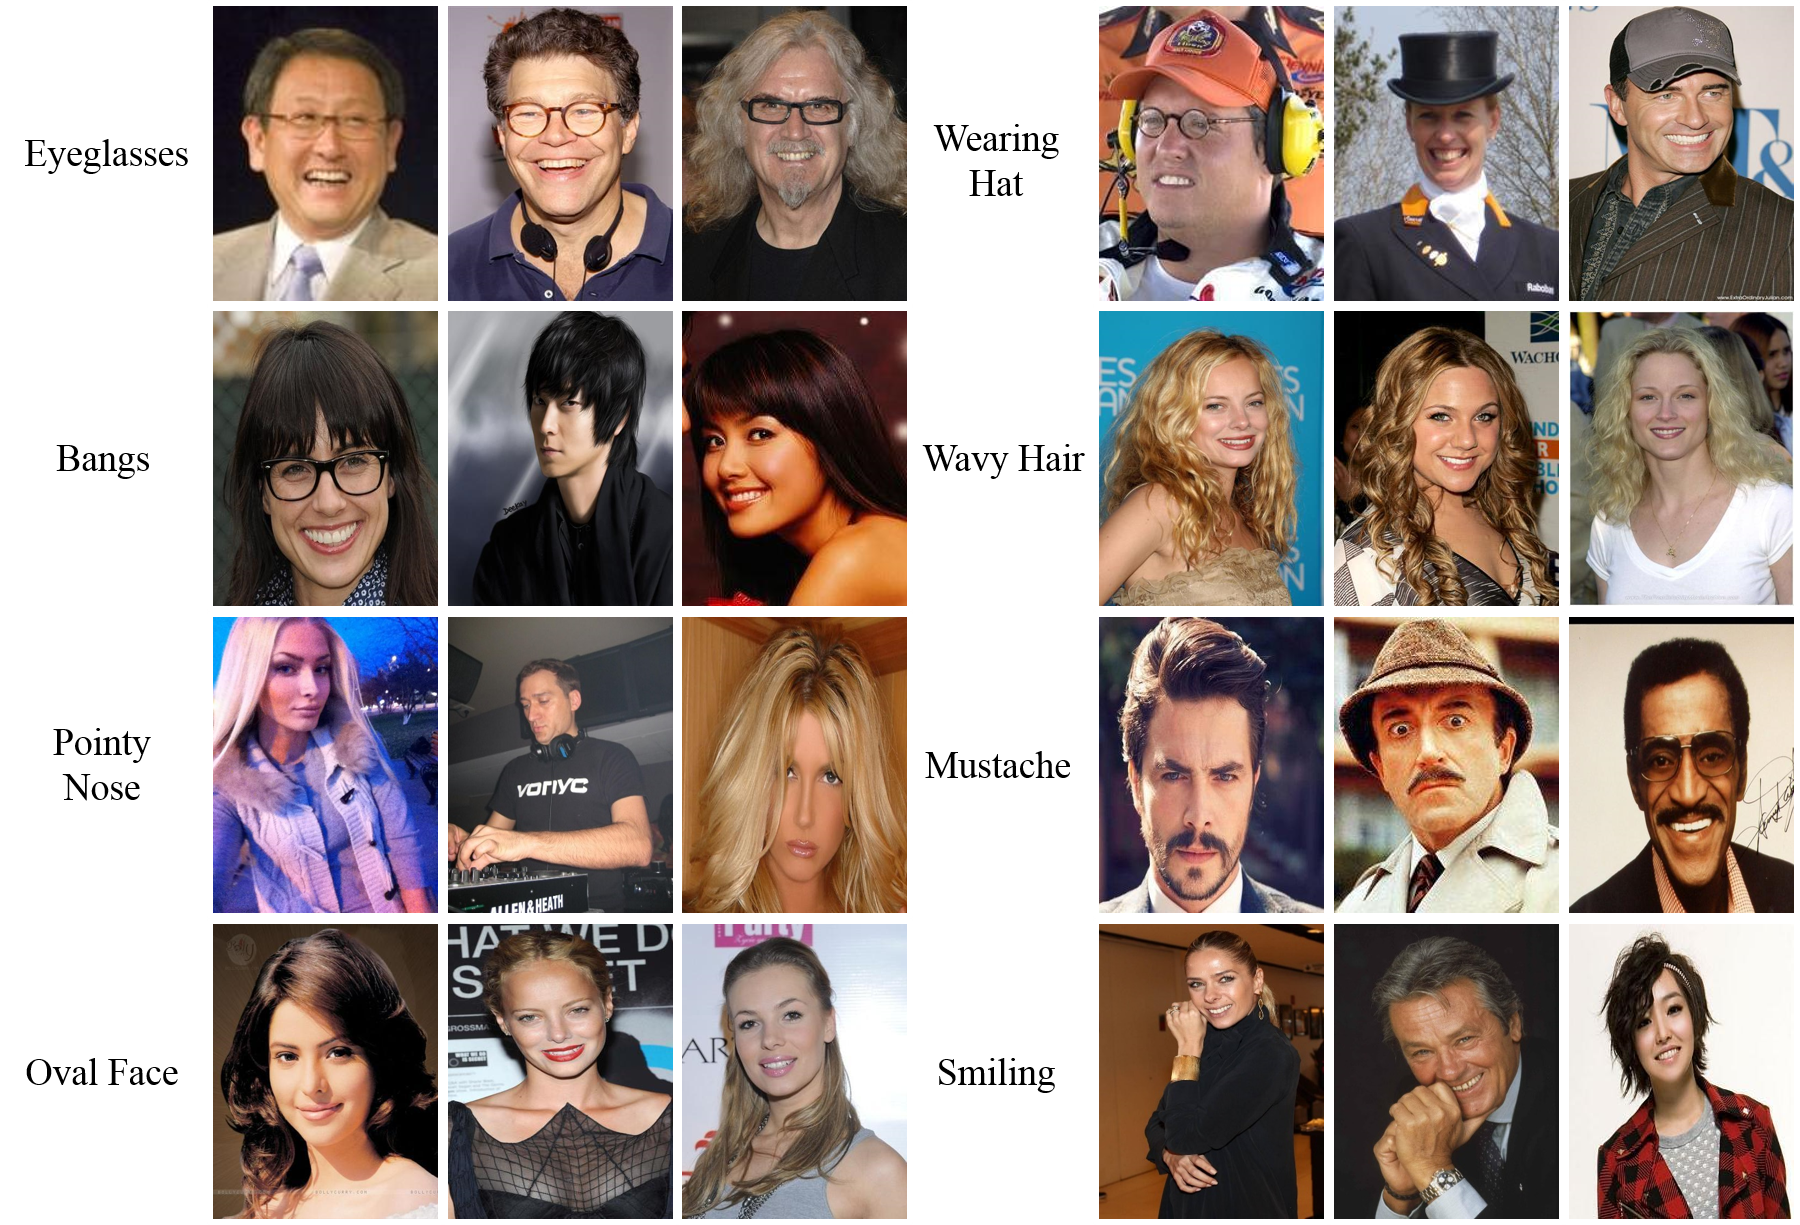
\includegraphics[width=0.5\textwidth]{CelebA}
\caption{CelebA dataset}
\label{fig:CelebA}
\end{figure}

CelebA is utilised as the face recognition model's dataset set in this project. The training set has 4429 photos while the test set has 1267 images.

\subsubsection{Private Dataset}

The private dataset consists of photos collected by team members. The photos were taken in SITE and feature various facial expressions.

This dataset is utilized to perform adversarial attacking on the face recognition model. The training set has 121 photos while the test set has 15 images.

\subsection{Faces extraction from recorded video}

After capturing three videos, OpenCV2 is used to sample 40 frames from each video. The faces are then rotated 180 degrees to accommodate package mediapipe's face detection model. Then, we crop the faces from the frames using the centre of the bounding box's coordinates. The faces are then saved in a folder named \verb|private_dataset| and added to \verb|CelebA_HQ_facial_identity_dataset|.

This process is done in \verb|Data_generation.ipynb.ipynb|.


\subsection{Associate id with name}

After downloading the CelebA dataset from the official website, we utilise CelebA-HQ-to-CelebA-mapping.txt to generate a map \verb|hq_A_mapping| from an id to the image file name, such as \verb|5: 000615.jpg|.
Then, we use list\_identity\_celeba.txt to generate the second map \verb|id_name_mapping| from a file name to its corresponding identity's name, for instance: \verb|000615.jpg: Martha Hunt|.

The benefit of this process is that we can now use the id to determine an identity's name. By example, we may use the following code: \verb|id_name_mapping[hq_A_mapping['5']]| to determine the name of the individual with id = 5.

This process is done in \verb|Preprocessing.ipynb|.

\subsection{Transforming the dataset}

We resized the images to 224x224 because their original size was too large for our model, which could cause performance issues. After that, we augment the tensor by giving it a random horizontal flip as part of the transformation.

This process is a part of \verb|simple_model.ipynb|.
